\begin{problem}%
{Шахматная доска}%
{\textsl{стандартный ввод}}%
{\textsl{стандартный вывод}}%
{2 секунды}%
{256 мегабайт}{}

Аня разделила доску размера $m \times n$ на клетки размера $1 \times 1$ и раскрасила их в черный и белый цвет в шахматном порядке. Васю заинтересовал вопрос: клеток какого цвета получилось больше — черного или белого.\\

Для того, чтобы выяснить это, он спросил у Ани, в какой цвет она раскрасила $j$-ю клетку в $i$-м ряду доски. По этой информации Вася попытался определить, клеток какого цвета на доске больше.\\

Требуется написать программу, которая по размерам доски и цвету $j$-й клетки в $i$-м ряду определит, клеток какого цвета на доске больше — черного или белого.

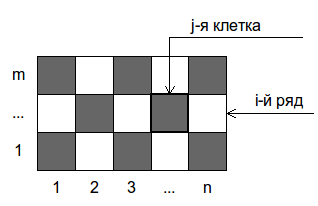
\includegraphics[scale=0.5]{images/3.png}

\InputFile

Входной файл содержит пять целых чисел: $m$, $n$, $i$, $j$ и $c$ ($1 \le m, n \le 10^9$, $1 \le i \le m$, $1 \le j \le n$, $c = 0$ или $c = 1$). Значение $c = 0$  означает, что $j$-я клетка в $i$-м ряду доски раскрашена в черный цвет, а значение $c = 1$  — в белый цвет.

\OutputFile

Выходной файл должен содержать одно из трех слов:

\begin{itemize}
\item \textit{black}, если черных клеток на доске больше,
\item \textit{white}, если белых клеток на доске больше,
\item \textit{equal}, если черных и белых клеток на доске поровну.
\end{itemize}

\Examples

\begin{example}
\exmp{
3 5 1 1 0
}{%
black
}%
\exmp{
3 5 2 1 0
}{%
white
}%
\exmp{
4 4 1 1 1
}{%
equal
}%
\end{example}
\end{problem}